\subsection{Data Memory}
\begin{figure}[!ht]
    \centering
    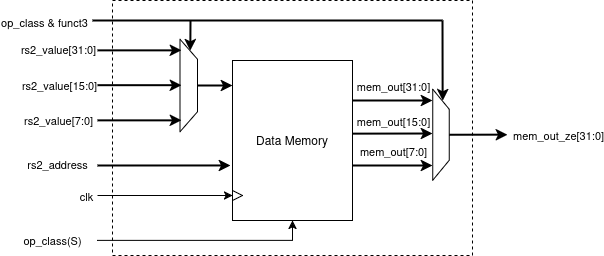
\includegraphics[scale = 0.45]{MEM_BD.png}
    \caption{DM interface block diagram}
    \label{fig:DM_BD}
\end{figure}

The final pieces that remain to be designed are the one that manages the Data Memory, and decides when to write, and the stage which, depending on the operation type, selects what to return as new value for the PC and what to store in the destination register, i.e the Write Back.\\
The Data Memory will instantiated as a 16KB single port RAM and separated from the rest, forming a 5-stage datapath when it is going to be pipelined. In 4-stages architecture it would be instead included in the same block, reducing the overall size of the processor, reducing power consumption, due to the presence of one less register, but at the cost of a reduced throughput.\\
The Table \ref{table:core_instr} indicates that there are many ways to perform L/S instruction and not only 32-bit vectors are handled. In fact some of them could manage just bytes or half-words, leaving some other options to be managed when executing these instructions. This discrimination cannot be performed by the ALU nor the Decoder, but it is easy to implement as interface for the Data Memory.
To be more specific, another case statement can be deployed to select filter the input and output of and from the memory, leaving the discrimination to both \emph{op{\_}class}, to see if an L/S operation is being performed, and \emph{funct3} to classify if the latter is working with bytes, half-words or words.

\subsection{Write Back}
\begin{figure}[!ht]
    \centering
    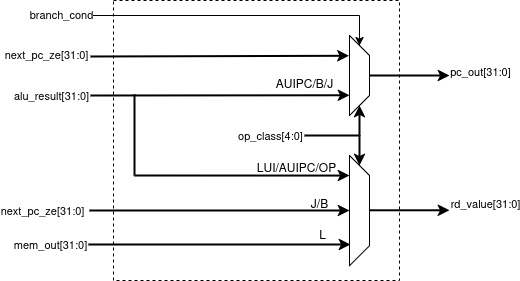
\includegraphics[scale = 0.45]{WB_BD.png}
    \caption{Write Back block diagram}
    \label{fig:WB_BD}
\end{figure}

The final step of execution, where the destination register and the program counter are written, needs a selector to decide what has to be overwritten and where; In the case of the PC two options can be identified: PC + 4 or the result from the ALU, which happens in case of a jump, a true condition from a branch or AUIPC. The destination register instead can be: the output of the ALU for classes OP, LUI, UIPC, PC + 4 for jumps and branches (when a logic high is returned, otherwise a high impedance output can be returned) or the output from the data memory. Source Code \ref{code:WB_code} shows again a case statement enclosed in an input-sensitive process, that is, a simple combinatory network.

\subsection{Simulation and final consideration}
With all the code prepared, the final simulation of the unpipelined datapath can be performed; Leaving the load-enable of the PC high, for there is no need to stall the execution for now, it is noticeable that the overall behavior corresponds to what is expected from it, although with a small concerning bug:

\begin{figure}[!ht]
    \centering
    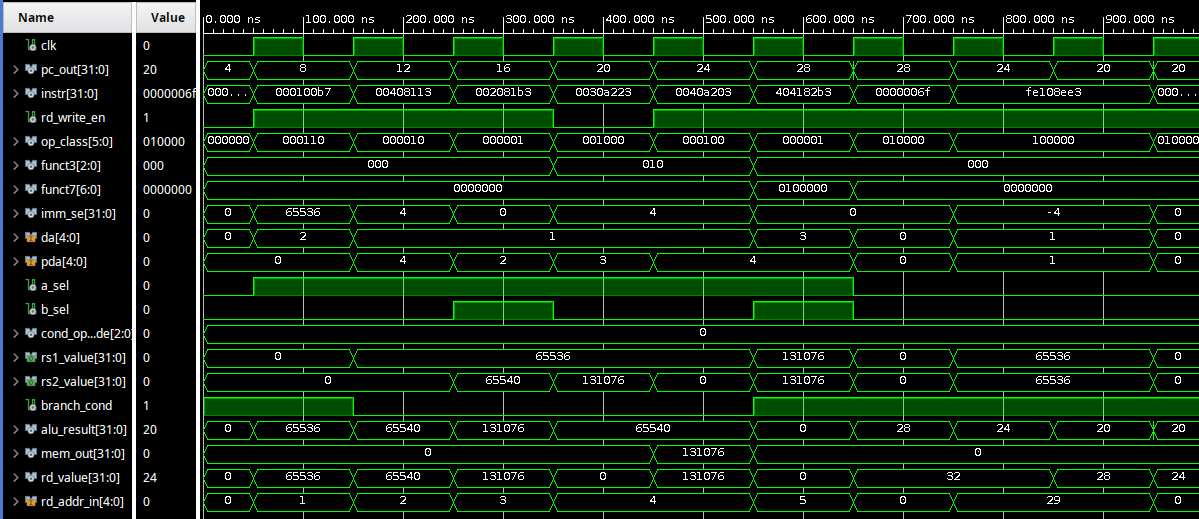
\includegraphics[scale = 0.36]{WB_sim.png}
    \caption{Complete simulation if the unpipelined datapath}
    \label{fig:WB_sim}
\end{figure}

Now L/S operations can effectively interact with the memory, although not each one of them has been tested. Also jumps and branches, with the output value for the PC being routed back to its original register, can move between instructions without problems.\\
A the very end of this basic implementation there are more some considerations to be made. For example x0 \emph{must not} be writable, instead all bits should be hardwired to a logic low, if not possible, then every attempt to write onto that must be ignored.\\
Another thing to observe from the code is that the multiplexer which selects between \emph{rs1} and \emph{rd}, at the end of the cycle will be left to '1', but since the architecture hasn't yet been pipelined, at the end of the operation the destination register cannot be overwritten, because the register file is only read and written during the rising edge of the clock, also during the next instruction, the resource has to be kept free. This is the first \emph{structural hazard} that this architecture is facing, leaving the only option to either stall the datapath for an amount of time after the execution cycle has terminated or implementing a pipeline, that is, having the processes of every stage sensitive to the rising edge of the clock instead of the inputs, meaning that every output is refreshed at that edge, as it would be expected by a register.